\begin{figure}[h]
\centering
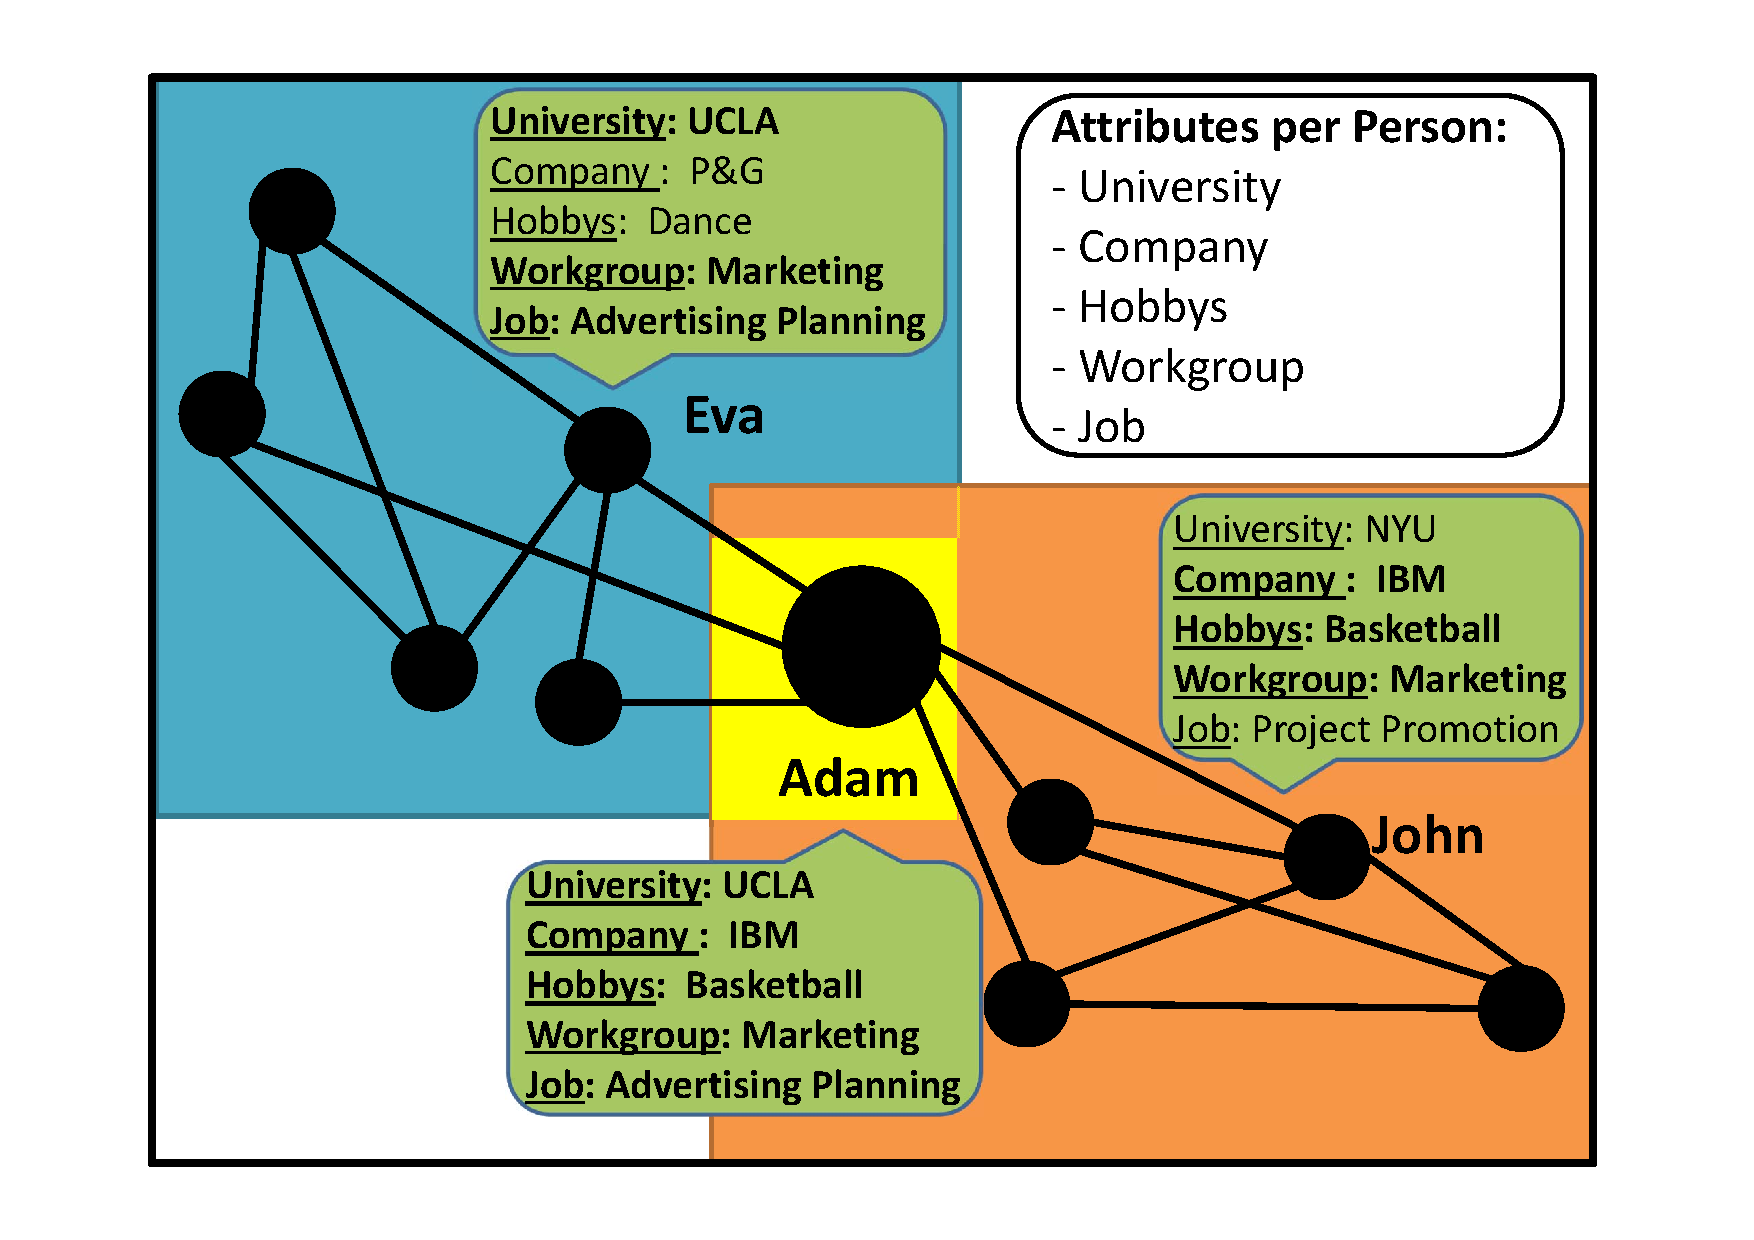
\includegraphics[width = 0.8\columnwidth]{figure/example.pdf}
\caption{Motivational example of a social friendship network.}
\label{fig:a}
\end{figure}

\section{Introduction}
Social networks, gene-and/or protein interaction networks as well as nearly all common types of networks in real world applications are not only sharing a large amount of information depending on the relationship between the vertices, but also contribute information regarding the characteristics of these vertices. These characteristics are modeled as attributes of a graphs' vertex. Thus we are referring to a graph containing extra information in its nodes as an \emph{attributed graph}. These attributed graphs connect two aspects of information: First, the structural "who knows whom" connection given by the graph itself as for example in friendship relationships of applications like facebook. Second, the attributes per node or person showing (in the case of facebook) personal ego-information like hobbys, what they are working, where they are living etc. Combining both aspects of information gives the chance to analyze things like "what has this friendship circle in common" or "what do most people in my work environment like and what joins them together?". Questions like this can be answered to some extend by just clustering attributed graphs, as existing algorithms propose in \cite{DBLP:conf/icdm/ZhouCY10}, \cite{DBLP:conf/sigmod/XuKWCC12} and \cite{DBLP:journals/pvldb/ZhouCY09}. But we are not only clustering attributed graphs but are also applying an overlapping concept to both informational aspects - to the graph structure and to the attribute space. What do we mean by overlapping and what do we gain out of the attributed graph if we are already able to group both informational aspects by just partitioning the attributed graph?


% what exactly does overlapping mean?

%Consider the fun example given in  Fig.\ref{fig:a} to outline the meaning of "overlapping" in combination with attributed graphs. It shows the friendship circle of a person called "Adam", he connects to people from his work environment and to people from outside his work environment that are still more or less living nearby like in the same city. The distance of the city-nodes to Adam visualizes how close they live together. Every person has the attributes of where he lives in, where he works and what hobbys he or she has. You could also think of the hobbys as more of a list, containing several attributes and differing in detail. Our Adam is living in detail in Vancouver, works at Eden Garden Center and likes skydiving as a hobby. The overlapping of the at least three dimensional attribute space and its corresponding friendship links is visualized in colored rectangles behind the graph structure. People in the same work environment likely know each other more than people from just the same city. We take a look at the two named nodes Lillith and Eva. Lillith is a working partner of Adam, living in the same city who shares some hobbys with him, lets say they even share skydiving. Let Eva be Adams' girlfriend living also close to Adam and sharing some interests, but not necessarily working together. Now, how would an attributed graph partitioner most likely divide this structure if no overlap is allowed? A possibility would be that Lillith is grouped together with the other working partners of Adam, creating a nearly full clique and therefore high quality in terms of clustering. Her share of hobbys with Adam and even Eva might be lost. With overlapping, Lillith being present in several communities would not only be in the one with the working people but also in a subspace cluster containing all people with similar hobbys (and living nearby) like Eva and Adam. She is also present in a very small connected group but highest dimensional attribute space in terms of all people that work together and have similar hobbys consisting only of Lillith and Adam. All in all this small example already shows the range of interpretability and complexity reduced from real world data when overlapping is not integrated.

Consider the example given in Fig.\ref{fig:a}, it outlines the meaning of ``overlapping" in combination with an attributed graph. The figure shows the friendship circles in a social network of a person called ``Adam". 
%He connects to people from the company he has worked in and to people who has studied in the same university with him. 
His two friendship circles are visualized in colored rectangles behind the graph structure: blue stands for his friends from school and orange indicates his circle of colleagues. The overlapping of both circles is highlighted in yellow. Every person (node) includes attributes on their university,  their working place and department, what hobbies they have and what job position they are in. % or she has studied, which company he or she works for, what hobbies he or she has, which department he or she works in and what type of job he or she does. 
You could also think of these attributes as more of a list, containing several items and differing in detail.
For example, Adam graduated from UCLA, works in IBM, likes playing basketball, works in the marketing department and is mainly in charge of planning advertisements. Now, how would an attributed graph partitioner most likely divide this structure if no overlap is allowed? A distinct possibility is to assign Adam to either the blue or the orange circle, because Adam can form a nearly full clique with both circles. This would result in a very high quality for clustering for one cluster while the other would lose some information (Adam). In this frequent case, partitioning must sacrifice the quality of this one cluster. Obviously, overlapping clustering, like assigning Adam to both circles, provides more meaningful structural information. Lets take a look at the two named nodes John and Eva that share some overlap in their attributes with Adam. John is a working partner of Adam, and shares the same hobby, workgroup and of course company with him. Also Eva graduated from the same university, shares the same workgroup and is working in a similar job like Adam, just in a different company. Therefore, Adam shares similar subspace attributes with his work circle where John is, while he shares other subspace with his school circle where Eva is. Apparently Adam should be assigned to both circles from the attribute information side as well.
%Besides, both John and Eva overlap with Adam on their workgroup, thus indicating the overlap different friendship clusters may representing a small connected cluster even though they are present in different friendship circles. Partitioning the graph structure would never reveal this small cluster. 
All in all this small example already shows the range of interpret-ability and complexity reduced from real world data when overlapping is not integrated.

%And he would not only be in the one with the people working in same workgroup of same company and even with same hobby, but also be a member of the one with people studying in same university and engaging in same job in same type of workgroup. Thus, overlapping (``Workgroup") also exists among detected coherent attributes which convey the meaning of the cluster.  

Therefore, we contribute a new method of clustering attributed graphs with the objective to find the reasonable overlapping communities and meaningful subspace of the attributes at the same time based on an information theoretical technique. The advantages of the proposed algorithm are in short:

\begin{itemize}
\item  \textbf{Discovery of overlapping communities}:
Our meth\\-od discovers not only single dense groups of friends but also their connections to other groups. Node structures can have several group memberships and be efficiently evaluated.
\item  \textbf{Finding coherent attribute subspaces}:
We think that some information is hidden in attribute subspaces that can be obtained to express the meaning of the cluster. Overlapping is also allowed among attribute subspaces.  
\item  \textbf{Without Redundancy}: 
Based on the Minimum Description Length (MDL) principle \cite{mdlbook}, our approach balances quality and redundancy in both graph structure and attribute space. Specifically, a node is only assigned to several graph clusters and an attribute is only part of multiple subspaces if this pays-off in terms of data compression. Thereby, only the truly relevant overlap useful to compress the data is reported as a result of our algorithm.
\item  \textbf{Automation}:
Our information theoretic based algorithm relieves the user from the task of finding parameters to run the method on every specific data. The non-redundant overlapping clusters and coherent attribute subspace can be detected automatically.  
%Basically we only need to retrieve one parameter specifically from the data, this parameter is of course evaluated in the experiments section, to show its very robust and thus it is possible to be chosen automatically.
\end{itemize}

The remainder of this paper is organized as follows: In the following section, we elaborate our coding scheme, which is necessary to avoid parametrization and balances among quality and redundancy. Section 3 describes the algorithm in detail. Section 4 shows experiments and results. Related work is discussed in Section 5. The conclusion follows in Section 6.

%With increasing complexity of data, graph has not sticked to only convey structural relation between vertices. A vertex if considered as an independent object contains information describing its character. For example,   Community detection is a significant task in mining graph data. Transitionally,  However, attributes plays a pivotal role in discovering knowledge from data as well. With the assistant of node attributes, more
% data element is able to possess multiple intimate connections to other data elements especially for graph data.  Therefore, overlapping exists between communities.
%
%In this paper, we proposed an information theoretic based algorithm which not only detects communities of an attributed graph with overlapping vertices but also discovers coherent subspace of attributes. The mainly contributions of our algorithm is conveyed as follow.
%
%1. Overlapping community detection:
%
%
%2. Finding coherent attributes subspace

